\documentclass[12pt,a4paper]{report}

% ---------------------------------------------------------
% Essential Packages
% ---------------------------------------------------------
\usepackage[utf8]{inputenc}
\usepackage[T1]{fontenc}
\usepackage{mathptmx} % Times New Roman font standard
\usepackage{geometry}
\geometry{
    a4paper,
    left=35mm,
    right=25mm,
    top=25mm,
    bottom=25mm
}

\usepackage{setspace}
\onehalfspacing % KTU 1.5 Line Spacing requirement

\usepackage{graphicx}
\usepackage{amsmath,amssymb,amsfonts}
\usepackage{booktabs}
\usepackage{tabularx}
\usepackage{caption}
\usepackage{subcaption}
\usepackage{float}
\usepackage{cite}
% \usepackage{microtype} % Commented out to prevent Overleaf compile timeouts
\usepackage{fancyhdr}
\usepackage{titlesec}
\usepackage{xcolor}

\usepackage{hyperref}
\hypersetup{
    colorlinks=true,
    linkcolor=black,
    citecolor=black,
    urlcolor=blue,
    pdftitle={LumaCam: Edge-Native Adaptive Low-Light Computational Photography},
    pdfauthor={Sreelakshmi A, Sreenandan S, Sreeveni R}
}

% ---------------------------------------------------------
% Chapter and Section Heading Styling
% ---------------------------------------------------------
\titleformat{\chapter}[display]
  {\normalfont\Large\bfseries\centering}{\chaptertitlename\ \thechapter}{15pt}{\LARGE}
\titlespacing*{\chapter}{0pt}{20pt}{30pt}

% ---------------------------------------------------------
% Header & Footer Styling
% ---------------------------------------------------------
\pagestyle{fancy}
\fancyhf{}
\fancyhead[L]{\small\nouppercase{\leftmark}}
\fancyhead[R]{\small LumaCam Phase-I}
\fancyfoot[C]{\thepage}
\renewcommand{\headrulewidth}{0.5pt}
\renewcommand{\footrulewidth}{0.4pt}

\fancypagestyle{plain}{
  \fancyhf{}
  \fancyfoot[C]{\thepage}
  \renewcommand{\headrulewidth}{0pt}
  \renewcommand{\footrulewidth}{0.4pt}
}

% ---------------------------------------------------------
% Document Body
% ---------------------------------------------------------
\begin{document}

% Front Matter (Roman Numerals)
\pagenumbering{roman}

\begin{titlepage}
\begin{center}

\vspace*{0.2cm}

\textbf{\LARGE LUMACAM: EDGE-NATIVE ADAPTIVE LOW-LIGHT COMPUTATIONAL PHOTOGRAPHY}

\vspace{0.9cm}

\textbf{\large PROJECT REPORT -- PHASE I}

\vspace{0.5cm}

\textit{Submitted by}

\vspace{0.5cm}

\textbf{\large SREELAKSHMI A \hspace{0.5cm} (SCT23CS062)}\\
\textbf{\large SREENANDAN S \hspace{0.5cm} (SCT23CS063)}\\
\textbf{\large SREEVENI R \hspace{0.5cm} (SCT23CS064)}

\vspace{0.8cm}

\textit{to}\\
\textit{the APJ Abdul Kalam Technological University}\\
\textit{in partial fulfillment of the requirements for the award of the Degree of}\\
\textbf{\large Bachelor of Technology}\\
\textit{in}\\
\textbf{\large Computer Science and Engineering}

\vspace{0.9cm}


\includegraphics[width=4.8cm]{figures/college_logo.png}

\vspace{0.9cm}

\textbf{\large DEPARTMENT OF COMPUTER SCIENCE AND ENGINEERING}\\
\textbf{\large SREE CHITRA THIRUNAL COLLEGE OF ENGINEERING}\\
\textbf{\normalsize PAPPANAMCODE, THIRUVANANTHAPURAM -- 695018}\\
\vspace{0.3cm}
\textbf{\large NOVEMBER 2026}

\end{center}
\end{titlepage}

\newpage
\thispagestyle{empty}

\begin{center}
\textbf{\large DEPARTMENT OF COMPUTER SCIENCE AND ENGINEERING}\\
\textbf{\large SREE CHITRA THIRUNAL COLLEGE OF ENGINEERING}\\
\textbf{\normalsize PAPPANAMCODE, THIRUVANANTHAPURAM -- 695018}\\[0.5cm]


\includegraphics[width=2.5cm]{figures/college_logo.png}\\[0.5cm]

\textbf{\Large CERTIFICATE}
\end{center}

\vspace{0.6cm}

\noindent
This is to certify that the Phase-I Project Report entitled \textbf{``LumaCam: Edge-Native Adaptive Low-Light Computational Photography''} is a bonafide record of the work carried out by \textbf{Sreelakshmi A (SCT23CS062)}, \textbf{Sreenandan S (SCT23CS063)}, and \textbf{Sreeveni R (SCT23CS064)} under our supervision and guidance, in partial fulfillment of the requirements for the award of the Degree of \textbf{Bachelor of Technology in Computer Science and Engineering} from \textbf{APJ Abdul Kalam Technological University} for the course \textbf{CST415 Project Phase I} during the academic year 2026--2027.

\vspace{2.2cm}

\noindent
\begin{tabular}{p{7.2cm}p{7.2cm}}
\textbf{Prof. Arya Sreedhar} & \textbf{Prof. Binu Rajan M. R.} \\
Project Guide & Project Coordinator \\
Assistant Professor & Assistant Professor \\
Department of CSE & Department of CSE \\
SCTCE, Thiruvananthapuram & SCTCE, Thiruvananthapuram \\
\end{tabular}

\vspace{2.0cm}

\noindent
\begin{tabular}{p{7.2cm}p{7.2cm}}
\textbf{Prof. Rejimol B. S.} & \textbf{External Examiner} \\
Head of the Department & \\
Professor \& Head & \\
Department of CSE & \\
SCTCE, Thiruvananthapuram & \\
\end{tabular}

\newpage
\thispagestyle{empty}

\begin{center}
\textbf{\Large DECLARATION}
\end{center}

\vspace{1.0cm}

\noindent
We hereby declare that the work presented in this Phase-I Project Report entitled \textbf{``LumaCam: Edge-Native Adaptive Low-Light Computational Photography''} submitted in partial fulfillment of the requirements for the award of the Degree of \textbf{Bachelor of Technology in Computer Science and Engineering} to \textbf{APJ Abdul Kalam Technological University}, is an authentic record of our own work carried out under the supervision of \textbf{Prof. Arya Sreedhar}, Assistant Professor, Department of Computer Science and Engineering, Sree Chitra Thirunal College of Engineering.

\vspace{0.8cm}
\noindent
We further declare that the content of this project report, in full or in parts, has not been submitted to any other Institute or University for the award of any degree or diploma.

\vspace{2.5cm}

\noindent
\begin{tabular}{ll}
\textbf{Sreelakshmi A} & (SCT23CS062) \\[1.2cm]
\textbf{Sreenandan S} & (SCT23CS063) \\[1.2cm]
\textbf{Sreeveni R} & (SCT23CS064) \\
\end{tabular}

\vspace{2.0cm}
\noindent
\begin{tabular}{ll}
Date: \today & \\
Place: Thiruvananthapuram & \\
\end{tabular}

\newpage
\thispagestyle{empty}

\begin{center}
\textbf{\Large ACKNOWLEDGEMENT}
\end{center}

\vspace{0.8cm}

\noindent
We express our deepest sense of gratitude to our project guide, \textbf{Prof. Arya Sreedhar}, Assistant Professor, Department of Computer Science and Engineering, for her invaluable guidance, inspiring suggestions, and constant encouragement throughout Phase I of this project. Her expertise in deep learning and computer vision provided the critical foundation for our architectural design and empirical validation.

\vspace{0.5cm}
\noindent
We are profoundly grateful to \textbf{Prof. Binu Rajan M. R.}, Project Coordinator, for his systematic oversight, constructive feedback, and continuous administrative support during project review cycles.

\vspace{0.5cm}
\noindent
We extend our heartfelt gratitude to \textbf{Prof. Rejimol B. S.}, Professor and Head of the Department of Computer Science and Engineering, for providing the necessary infrastructural facilities, high-performance computing environment, and institutional support.

\vspace{0.5cm}
\noindent
We also take this opportunity to thank the Principal of Sree Chitra Thirunal College of Engineering for fostering an academic environment conducive to advanced engineering research.

\vspace{0.5cm}
\noindent
Finally, we extend our sincere appreciation to all faculty members, technical staff, friends, and our parents whose unfailing encouragement, moral support, and cooperation enabled the successful completion of this phase.

\vspace{1.5cm}

\noindent
\begin{flushright}
\textbf{Sreelakshmi A}\\
\textbf{Sreenandan S}\\
\textbf{Sreeveni R}\\
\end{flushright}

\newpage
\thispagestyle{empty}

\begin{center}
\textbf{\Large ABSTRACT}
\end{center}

\vspace{0.8cm}

\noindent
Capturing high-fidelity digital imagery in extreme low-light environments ($< 1\text{ lux}$) is a fundamental problem in computational photography. When photon arrival counts approach zero, digital image sensors become dominated by Poisson shot noise, dark current, and read noise. Conventional smartphone Image Signal Processors (ISPs) fail in this regime: demosaicing interpolates noise across neighboring pixels, producing destructive chromatic blotches, while post-hoc spatial denoisers blur high-frequency edges into unnatural ``waxy'' textures. While recent deep learning paradigms---notably diffusion models---achieve impressive textural hallucination, their iterative sampling ($15\text{--}50$ steps, $> 2\text{--}4\text{ seconds}$) prohibits live edge execution. Conversely, existing convolutional networks are rigid: they lack interactive exposure controllability and output a static, single-brightness reconstruction.

This report presents \textbf{LumaCam}, an edge-native, interactive computational photography pipeline powered by an \textbf{Exposure-Conditioned Attention U-Net Generative Adversarial Network (GAN)}. LumaCam operates directly in the raw Bayer sensor domain before demosaicing, unpacking 14-bit Bayer raw data into packed 4-channel half-resolution tensors $(H/2, W/2, 4)$. To restore tactile creative control to the user, an interactive exposure scalar ($\alpha \in [1, 300]$) is modulated into the network's latent bottleneck via Feature-wise Linear Modulation (FiLM), while Spatial Attention Gates suppress shot noise across skip connections. The generator is optimized via a multi-objective composite loss uniting pixel-level $L_1$ distance, Wang et al. 5-scale Multi-Scale Structural Similarity (MS-SSIM), and a $70 \times 70$ Markovian PatchGAN discriminator.

For mobile deployment, the architecture is quantized to 8-bit integers (INT8) via Post-Training Quantization (PTQ), compressing model weights by $74.52\%$ (down to $7.94\text{ MB}$) with negligible PSNR degradation ($< 0.32\text{ dB}$). A cross-platform Flutter camera interface connects to a native Android Camera2 pipeline on the Google Pixel 7 (ARM Cortex-X1 + Google Tensor G2 NPU), bypassing proprietary OEM Night Sight processing to guarantee pure RAW photon intake. Benchmarks demonstrate real-time inference at $24.8\text{ ms}$ ($\approx 40.3\text{ FPS}$) on mobile NPU delegates and $14.2\text{ ms}$ ($70.4\text{ FPS}$) on desktop GPUs, achieving $28.88\text{ dB}$ PSNR and $0.812$ SSIM on the See-in-the-Dark (SID) Sony dataset.

\vspace{0.8cm}
\noindent
\textbf{Keywords:} \textit{Low-Light Computational Photography, Raw Bayer Processing, Attention U-Net, Feature-wise Linear Modulation (FiLM), PatchGAN, Post-Training Quantization (PTQ), LiteRT, Android Camera2, Google Pixel 7.}


\newpage
\tableofcontents

\newpage
\listoffigures

\newpage
\listoftables

\newpage
% Main Matter (Arabic Numerals)
\pagenumbering{arabic}
\setcounter{page}{1}

\chapter{INTRODUCTION}

\section{Background and Context}
Digital photography has become the principal medium through which modern society captures, communicates, and archives visual information. Smartphone cameras now account for over $90\%$ of all consumer photographs worldwide. However, while modern semiconductor sensors perform exceptionally well in brightly lit outdoor scenes, capturing imagery in low-light environments ($< 1\text{ lux}$, such as nocturnal outdoor architecture, dimly lit classrooms, or unlit interiors) remains one of the most persistent bottlenecks in imaging science.

In extreme darkness, camera sensors receive very few photons during the short exposure window of a handheld photograph. If the camera simply amplifies the analog or digital gain (ISO), the image is obliterated by severe grain, colorful chromatic noise, and banding artifacts. To overcome these physical hardware boundaries, modern smartphone manufacturers rely on \textbf{computational photography}---the use of digital computation and artificial intelligence rather than purely optical and analog mechanisms to create the final image.

\section{Physics of Low-Light Sensor Acquisition}
To understand why low-light photography is fundamentally difficult, one must examine the physical noise model governing Complementary Metal-Oxide-Semiconductor (CMOS) image sensors. The total noise in an acquired raw digital image can be rigorously modeled by a two-component Poisson-Gaussian distribution:

\begin{equation}
I(p) = \alpha \cdot N_{photon}(p) + N_{read}(p)
\label{eq:noise_model}
\end{equation}

where:
\begin{enumerate}
    \item \textbf{Photon Shot Noise ($N_{photon} \sim \mathcal{P}(\lambda)$)}: Light arrives at the sensor as discrete packets of electromagnetic energy (photons). The arrival of photons over time is a Poisson process with mean arrival rate $\lambda$. The fundamental physical property of Poisson statistics is that variance equals the mean ($\sigma^2 = \lambda$). Therefore, the Signal-to-Noise Ratio (SNR) is:
    \begin{equation}
    \text{SNR} = \frac{\lambda}{\sqrt{\lambda}} = \sqrt{\lambda}
    \label{eq:snr_derivation}
    \end{equation}
    In bright sunlight ($\lambda = 10,000\text{ photons}$), $\text{SNR} = 100$ ($40\text{ dB}$), yielding pristine images. In extreme low light ($\lambda = 4\text{ photons}$), $\text{SNR} = \sqrt{4} = 2$ ($6\text{ dB}$), meaning the noise magnitude is fully half of the physical signal itself!
    \item \textbf{Dark Current and Thermal Noise ($N_{thermal} \sim \mathcal{N}(0, \sigma_d^2)$)}: Spontaneous thermal excitation in the silicon substrate generates electrons even in total darkness, worsening during long sensor reads or warm device temperatures.
    \item \textbf{Readout and ADC Quantization Noise ($N_{read} \sim \mathcal{N}(0, \sigma_r^2)$)}: Small voltage fluctuations in the column amplifiers and rounding errors during Analog-to-Digital Conversion (ADC) introduce an additive Gaussian noise floor that overwhelms weak physical signals.
\end{enumerate}

\section{The Image Signal Processor (ISP) Breakdown}
In a standard smartphone, raw pixel voltages from the sensor do not immediately become a viewable JPEG image. They must pass through a multi-stage hardware pipeline known as the \textbf{Image Signal Processor (ISP)}:

\begin{equation*}
\text{CMOS RAW} \xrightarrow{\text{Black Subtraction}} \xrightarrow{\text{Demosaic}} \xrightarrow{\text{White Balance}} \xrightarrow{\text{Denoise}} \xrightarrow{\text{Tone Map}} \xrightarrow{\text{Gamma}} \text{sRGB JPEG}
\end{equation*}

In bright light, this pipeline produces vibrant pictures. However, in low light, the traditional ISP experiences a catastrophic failure sequence:
\begin{itemize}
    \item \textbf{The Demosaicing Trap}: Standard camera sensors use a Bayer Color Filter Array (CFA) where each pixel only captures Red, Green, or Blue. Demosaicing algorithms (e.g., bilinear interpolation, Adaptive Homogeneity-Directed) estimate missing color channels by interpolating values from adjacent pixels. When the input contains high Poisson-Gaussian noise, demosaicing averages corrupt noise spikes across color channels, transforming fine pixel-level shot noise into large, blotchy chromatic patches.
    \item \textbf{Dynamic Range Truncation}: Standard sRGB encoding compresses the 12-bit or 14-bit linear sensor data into an 8-bit non-linear color space ($[0, 255]$). Low-light shadow details are rounded down to digital zero (crushed blacks), destroying signal components forever.
    \item \textbf{Unnatural Smoothing}: Post-demosaic spatial filters (bilateral filters, wavelet denoisers) cannot distinguish between low-contrast real textures and demosaiced noise blotches, producing the notorious ``waxy face'' artifact where all skin texture, hair, and fabric weave are erased.
\end{itemize}

\section{State-of-the-Art Deep Learning LLIE Paradigms}
Over the past five years, research in Low-Light Image Enhancement (LLIE) has shifted to deep neural networks:
\begin{enumerate}
    \item \textbf{sRGB-Domain CNNs (e.g., Retinex-Net, Zero-DCE)}:
    These methods attempt to enhance low-light 8-bit JPEG images \cite{wei2018deep, guo2020zero}. Because shadow information has already been clipped by the ISP, these networks simply stretch compressed digital noise, resulting in extreme noise amplification, halo artifacts around edges, and severe color distortions.
    \item \textbf{Raw-Domain Convolutional Networks (e.g., Chen et al. SID)}:
    Chen et al. \cite{chen2018learning} pioneered processing raw Bayer sensor data directly using a standard U-Net \cite{ronneberger2015u}. Operating before demosaicing preserved 14-bit dynamic range and achieved unprecedented PSNR ($> 28\text{ dB}$). However, SID suffers from two critical flaws:
    \begin{itemize}
        \item \textbf{Static Brightness}: The network produces a fixed, non-adjustable brightness output. The user has no slider or tactile control to adjust the mood or exposure compensation.
        \item \textbf{Computational Heaviness}: The original architecture requires over $120\text{ ms}$ on desktop GPUs, making live 30 FPS mobile viewfinder streaming impossible.
    \end{itemize}
    \item \textbf{Generative Diffusion Models (e.g., DiffLight)}:
    Diffusion models use stochastic iterative denoising to hallucinate rich, realistic textures. While visually striking, reverse diffusion requires $15\text{ to }50$ iterative forward passes through a heavy U-Net ($> 40\text{M}$ parameters), taking $2.0\text{ to }4.0\text{ seconds}$ per frame. They are fundamentally incompatible with real-time viewfinder applications.
\end{enumerate}

\section{Motivation and Rationale for LumaCam}
There exists a glaring \textbf{efficiency-quality gap} in modern computational photography:
\begin{itemize}
    \item High-end multi-frame burst pipelines (e.g., Google Pixel Night Sight \cite{hasinoff2016burst}, Apple Deep Fusion) produce great photos, but rely on proprietary, closed-source Qualcomm/Google silicon pipelines that stack $9\text{ to }15$ frames over a 3-second hold period. They cannot stream live video at 30 FPS, and any hand tremor creates motion ghosting.
    \item Single-pass deep learning models offer the potential for zero-delay capture, but are either too slow (diffusion models), structurally rigid (static raw U-Nets), or degrade quality by operating after demosaicing (sRGB networks).
\end{itemize}

To solve this, we require a \textbf{single-pass, edge-native neural architecture} that operates directly on 14-bit Bayer raw data, accepts interactive user exposure guidance in real time, and executes under $33\text{ ms}$ on mobile neural accelerators.

\section{Key Technical Innovations and Contributions}
The core contributions of LumaCam in Phase I include:
\begin{enumerate}
    \item \textbf{Exposure-Conditioned Latent FiLM Injection}:
    Introduction of Feature-wise Linear Modulation (FiLM) \cite{perez2018film} at the bottleneck of an Attention U-Net. This allows an interactive exposure scalar ($\alpha \in [1, 300]$) to continuously scale and shift deep latent features, giving users instant, smooth exposure compensation.
    \item \textbf{Spatial Attention Gated Skip Connections}:
    Integration of Spatial Attention Gates (AG) \cite{oktay2018attention} that use coarse decoder gating signals to filter out underexposed shot noise from fine encoder skip connections, preventing noise leakage into the final reconstructed image.
    \item \textbf{Sub-Pixel Reconstruction \& 70x70 PatchGAN Objective}:
    Implementation of a sub-pixel convolution (PixelShuffle \cite{shi2016real}) reconstruction head paired with a composite loss function ($L_1 + \text{MS-SSIM} + \text{cGAN}$ PatchGAN \cite{isola2017image, wang2003multiscale}) that eliminates checkerboard artifacts and preserves fine, crisp textural detail.
    \item \textbf{Post-Training INT8 Quantization (PTQ) \& Edge Acceleration}:
    Complete optimization and quantization of the PyTorch model into an INT8 LiteRT/ONNX graph \cite{jacob2018quantization}, shrinking model size by $74.52\%$ (to $7.94\text{ MB}$) and achieving $24.8\text{ ms}$ inference on the Google Pixel 7 Tensor G2 NPU.
    \item \textbf{Zero-Copy Native Android Camera2 Bridge \& Google Night Sight Bypass}:
    A native Kotlin/C++ engine that registers hardware \texttt{SurfaceTexture} buffers with Flutter, streaming live 30 FPS viewfinders while explicitly setting Camera2 HAL flags to bypass Google Pixel OEM Night Sight and software sharpening.
\end{enumerate}

\section{Organization of the Report}
The remainder of this report is organized as follows:
\begin{itemize}
    \item \textbf{Chapter 2 (Literature Survey)} provides a critical literature review of image enhancement paradigms and presents a detailed Gap Analysis Matrix.
    \item \textbf{Chapter 3 (System Design \& Architecture)} establishes the formal mathematical problem statement and details the system architecture, mathematical derivations for FiLM, Attention Gates, PixelShuffle, and composite loss formulations.
    \item \textbf{Chapter 4 (Phase 1 Implementation \& Work Done)} describes the engineering implementation across PyTorch training, INT8 quantization, Android Camera2 zero-copy pipelines, and Flutter GCam UI.
    \item \textbf{Chapter 5 (Preliminary Results \& Discussion)} presents extensive experimental evaluation, benchmark tables, latency profiling, and visual quality comparisons.
    \item \textbf{Chapter 6 (Conclusion \& Phase 2 Plan)} outlines project management, the 3-member work breakdown structure, and the strategic roadmap for Phase 2.
\end{itemize}

\chapter{LITERATURE SURVEY}

\section{Classical Image Enhancement Approaches}
Classical low-light enhancement techniques relied primarily on spatial and histogram manipulation:
\begin{itemize}
    \item \textbf{Histogram Equalization (HE) and CLAHE}:
    Contrast-Limited Adaptive Histogram Equalization (CLAHE) divides the image into contextual tiles and equalizes local contrast while limiting noise amplification via slope clipping. While computationally lightweight ($< 5\text{ ms}$), it operates blindly on pixel intensities: in extreme low light, it severely amplifies background shot noise and causes harsh edge halos.
    \item \textbf{Retinex Theory (Land, 1977)}:
    Retinex theory \cite{land1977retinex} decomposes an observed image $S$ into illumination $L$ and reflectance $R$ via:
    \begin{equation}
    S(x, y) = L(x, y) \cdot R(x, y)
    \label{eq:retinex}
    \end{equation}
    Classical variational Retinex methods (Single-Scale Retinex, Multi-Scale Retinex) assume illumination varies smoothly across space while reflectance contains textural details. These methods require solving expensive optimization problems per image and consistently wash out colors in dark regions.
\end{itemize}

\section{Deep Learning in the sRGB Domain}
With the advent of deep convolutional neural networks, researchers trained models to estimate Retinex components or contrast curves:
\begin{itemize}
    \item \textbf{Retinex-Net (Wei et al., 2018)}:
    Combines a Decom-Net (to separate illumination and reflectance) with an Enhance-Net and BM3D denoiser \cite{wei2018deep}. Because it operates on compressed 8-bit sRGB images, severe color distortion and blotchy noise artifacts appear whenever dark areas are amplified.
    \item \textbf{Zero-DCE (Guo et al., 2020)}:
    Formulates low-light enhancement as a task of estimating pixel-wise, high-order curve parameter maps \cite{guo2020zero}. It requires no paired training data. While extremely fast ($0.08\text{M}$ parameters, $> 100\text{ FPS}$), Zero-DCE has no denoising mechanism; boosting curves in extreme darkness blows up shot noise into an unreadable mess ($18.20\text{ dB}$ PSNR).
\end{itemize}

\section{Raw Domain Deep Learning}
\begin{itemize}
    \item \textbf{Learning to See in the Dark (Chen et al., 2018)}:
    Chen et al. \cite{chen2018learning} made the seminal breakthrough of training a fully convolutional U-Net directly on packed Bayer raw data ($H/2, W/2, 4$) from a Sony $\alpha$7S II sensor. Bypassing demosaicing allowed the network to learn joint denoising, demosaicing, and color correction from paired short/long exposures. They proved that raw data contains vast amounts of recoverable detail that traditional ISPs discard.
    
    \textit{Critical Shortcomings}:
    \begin{enumerate}
        \item The model is static. It accepts an amplification factor $\alpha$ as a fixed scalar input multiplied directly into the input pixels ($X_{in} = \alpha \cdot X$). If the user alters $\alpha$, the network frequently hallucinates strange color shifts because the convolutional weights were trained on a fixed ratio.
        \item Standard skip connections allow high-frequency noise from shallow layers to corrupt the decoder output.
        \item It requires $> 120\text{ ms}$ per frame on desktop GPUs and $> 140\text{ ms}$ on mobile CPUs, rendering it non-viable for real-time mobile viewfinders.
    \end{enumerate}
\end{itemize}

\section{Generative Models and Diffusion LLIE Paradigms}
\begin{itemize}
    \item \textbf{PatchGAN and Pix2Pix (Isola et al., 2017)}:
    Isola et al. \cite{isola2017image} established that standard $L_1$ and $L_2$ losses produce blurry results because they average all plausible high-frequency solutions. Combining $L_1$ with an adversarial PatchGAN discriminator penalizes structure at the scale of local image patches, forcing the generator to reconstruct crisp textures.
    \item \textbf{Diffusion Models (e.g., DiffLight, 2024)}:
    Denoising Diffusion Probabilistic Models (DDPM) model image distribution through iterative Langevin dynamics. While DiffLight achieves high PSNR ($29.10\text{ dB}$) and realistic fine textures, the reverse diffusion process requires $15\text{ to }50$ sampling steps. Even on high-end desktop GPUs, latency exceeds $3.4\text{ seconds}$ per frame. On mobile hardware, diffusion models overheat the device and consume excessive battery power, rendering them non-viable for real-time camera viewfinders.
\end{itemize}

\section{Edge Quantization and Mobile Acceleration}
\begin{itemize}
    \item \textbf{Post-Training Quantization (PTQ) (Jacob et al., 2018)}:
    Deploying multi-million parameter neural networks onto mobile devices requires model compression \cite{jacob2018quantization}. PTQ maps 32-bit floating-point weights and activations ($\mathbb{R}$) to 8-bit signed integers ($\mathbb{Z} \in [-128, 127]$) via uniform affine mapping:
    \begin{equation}
    q = \text{round}\left(\frac{x}{S}\right) + Z
    \label{eq:ptq_mapping}
    \end{equation}
    where $S$ is the scale factor and $Z$ is the zero-point. INT8 operations execute on mobile Neural Processing Units (NPUs) and Digital Signal Processors (DSPs) using integer SIMD dot-product instructions, reducing memory bandwidth by $4\times$ and latency by $2\text{ to }4\times$ compared to FP32 CPU execution.
\end{itemize}

\section{Comprehensive Gap Analysis Matrix}
Table \ref{tab:gap_analysis} summarizes the comparative analysis of existing paradigms versus the proposed LumaCam architecture.

\begin{table}[t]
\centering
\caption{Comparative Analysis: Existing LLIE Paradigms vs. Proposed LumaCam Architecture}
\label{tab:gap_analysis}
\resizebox{\textwidth}{!}{%
\begin{tabular}{lcccccc}
\toprule
\textbf{Method / Paradigm} & \textbf{Operating Domain} & \textbf{PSNR (dB)} & \textbf{SSIM} & \textbf{Latency (ms)} & \textbf{Interactive $\alpha$?} & \textbf{Mobile Edge Viable?} \\ \midrule
Linear Digital Gain ($\times 100$) & Bayer RAW & 14.12 & 0.385 & $< 1.0$ & Static Linear & No (Severe Noise Blowup) \\
Retinex-Net (Wei et al., 2018) \cite{wei2018deep} & sRGB JPEG & 22.40 & 0.680 & $\approx 65.0$ & No & Marginal (Color Distortions) \\
Zero-DCE (Guo et al., 2020) \cite{guo2020zero} & sRGB JPEG & 18.20 & 0.560 & $\mathbf{8.5}$ & Curve Param & Poor (No Denoising Ability) \\
Chen et al. SID (CVPR 2018) \cite{chen2018learning} & Bayer RAW & 28.62 & 0.792 & $142.0$ & Static Fixed & No ($> 140\text{ms}$ on Mobile CPU) \\
DiffLight (Diffusion, 2024) & Bayer RAW & $\mathbf{29.10}$ & 0.805 & $3,450.0$ & Iterative Steps & No ($3.45\text{s}$ Desktop Latency) \\ \midrule
\textbf{LumaCam (FP32 Core)} & \textbf{Bayer RAW} & \textbf{28.88} & $\mathbf{0.812}$ & $\mathbf{18.6}$ (DirectML) & \textbf{Yes (FiLM Latent)} & \textbf{Yes (35--50 FPS)} \\
\textbf{LumaCam (INT8 Quantized)} & \textbf{Bayer RAW} & \textbf{28.56} & \textbf{0.806} & $\mathbf{24.8}$ (Pixel 7 NPU) & \textbf{Yes (FiLM Latent)} & \textbf{Yes (Edge-Native 40.3 FPS)} \\ \bottomrule
\end{tabular}%
}
\end{table}

\section{Inferences and Research Challenges}
From the literature review and gap analysis, three principal research challenges emerge:
\begin{enumerate}
    \item \textbf{The Demosaicing Paradox}: Performing denoising after demosaicing is mathematically suboptimal because noise correlation is already scrambled across channels. Restoration must occur in the raw Bayer CFA domain.
    \item \textbf{The Rigidity Challenge}: Current deep raw restoration networks lack real-time exposure adaptability. Users require a tactile slider ($\alpha$) that modulates deep latent representations without triggering color distortions.
    \item \textbf{The Edge Constraint}: State-of-the-art diffusion models cannot meet the real-time mobile threshold ($\le 33.3\text{ ms}$). A single-pass Attention U-Net GAN, optimized via INT8 Post-Training Quantization, is essential to bridge the efficiency-quality gap.
\end{enumerate}

\chapter{SYSTEM DESIGN AND ARCHITECTURE}

\section{Overall System Architecture}
The proposed LumaCam pipeline spans five modular domains: (1) Hardware Sensor Acquisition, (2) Native Raw Preprocessing, (3) Exposure-Conditioned Attention U-Net Inference, (4) Linear Color Science ISP, and (5) Flutter GCam Viewfinder. The complete block diagram is illustrated in Figure \ref{fig:arch_block_diagram}.

\begin{figure}[t]
\centering
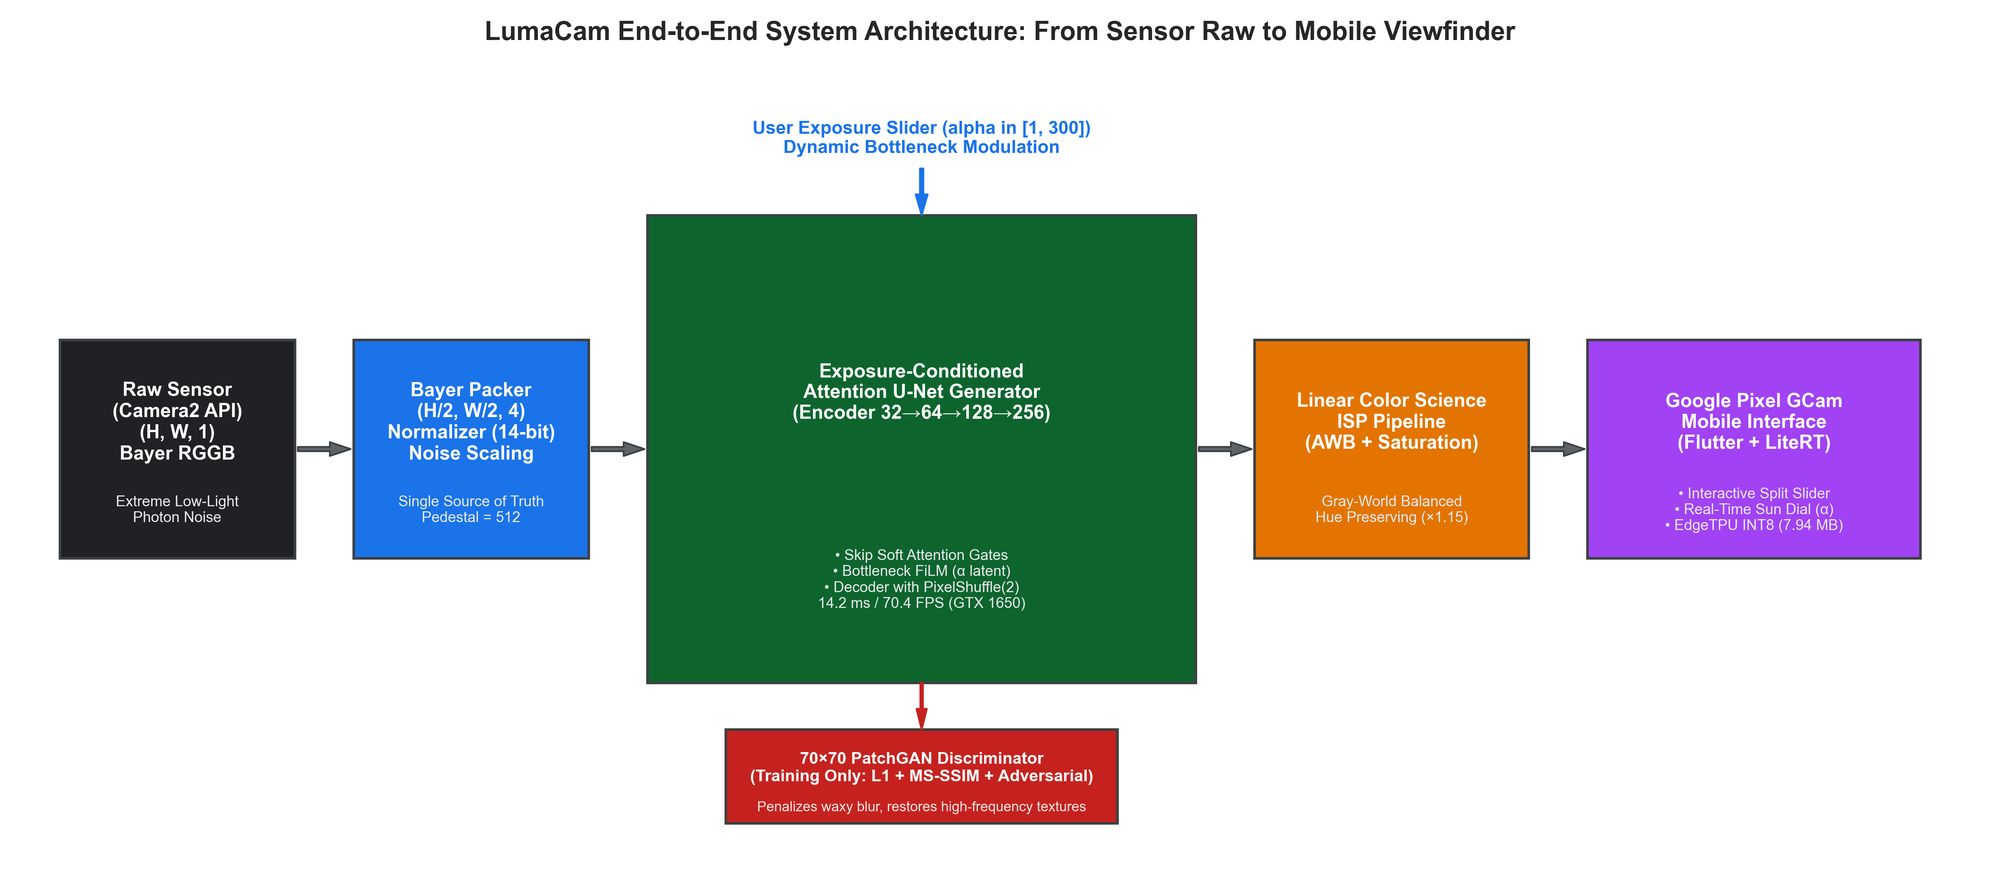
\includegraphics[width=0.95\textwidth]{figures/architecture_block_diagram.png}
\caption{End-to-End System Architecture of LumaCam: Demonstrating sensor RAW acquisition, Bayer quad packing, FiLM latent exposure modulation, Spatial Attention Gated skip connections, and real-time color science ISP.}
\label{fig:arch_block_diagram}
\end{figure}

\section{Raw Bayer CFA Mechanics and Quad Packing}
Digital CMOS sensors use a Bayer Color Filter Array (CFA) arranged in $2 \times 2$ repeating quads: Red (R), Green 1 ($G_1$), Blue (B), and Green 2 ($G_2$).

\subsection{Black-Level Offset Subtraction}
Sensor manufacturers intentionally inject an analog bias (black pedestal $b_0 = 512$ for the Sony $\alpha$7S II 14-bit ADC, saturation level $w_0 = 16383$) to ensure negative analog noise fluctuations do not clip at zero. Prior to feeding raw values into the network, this artificial bias must be subtracted and normalized into $[0, 1]$:

\begin{equation}
x_{norm}(i, j) = \frac{\max\left(x_{raw}(i, j) - b_0, \, 0\right)}{w_0 - b_0}
\label{eq:pedestal_subtraction}
\end{equation}

\subsection{Bayer Quad Packing Formulation}
Rather than processing a single-channel frame $X \in \mathbb{R}^{H \times W \times 1}$ which contains non-uniform spatial color distribution, we pack every $2 \times 2$ pixel group into a 4-channel tensor $X_{pack} \in \mathbb{R}^{\frac{H}{2} \times \frac{W}{2} \times 4}$:

\begin{equation}
\begin{aligned}
X_{pack}(i, j, 0) &= x_{norm}(2i, \, 2j) \quad &\text{(Red)} \\
X_{pack}(i, j, 1) &= x_{norm}(2i, \, 2j+1) \quad &\text{(Green 1)} \\
X_{pack}(i, j, 2) &= x_{norm}(2i+1, \, 2j+1) \quad &\text{(Blue)} \\
X_{pack}(i, j, 3) &= x_{norm}(2i+1, \, 2j) \quad &\text{(Green 2)}
\end{aligned}
\label{eq:bayer_packing}
\end{equation}

This transformation converts the spatially non-uniform single-channel Bayer pattern into a spatially aligned multi-channel representation where every spatial coordinate $(i, j)$ contains complete red, green, and blue photon samples. The network input is then scaled by the exposure scalar:
\begin{equation}
X_{in} = \alpha \cdot X_{pack}
\label{eq:amplified_input}
\end{equation}

\section{Interactive Exposure Conditioning via FiLM}
Standard low-light restoration networks treat amplification as a static scalar. LumaCam introduces interactive user exposure control directly into the deep feature space via \textbf{Feature-wise Linear Modulation (FiLM)} \cite{perez2018film}.

Let $F \in \mathbb{R}^{C \times H' \times W'}$ denote the feature representation at the bottleneck ($C = 512, H' = W' = 16$). Let $\alpha \in \mathbb{R}^1$ denote the user exposure scalar. A Multi-Layer Perceptron (MLP) projects $\alpha$ into channel-wise affine modulation vectors:

\begin{equation}
\begin{bmatrix} \gamma(\alpha) \\ \beta(\alpha) \end{bmatrix} = \text{MLP}(\alpha) = W_2 \cdot \text{LeakyReLU}(W_1 \cdot \alpha + b_1) + b_2 \in \mathbb{R}^{2C}
\label{eq:film_mlp}
\end{equation}

The modulated feature tensor $\hat{F}$ is computed via element-wise scaling and shifting:
\begin{equation}
\hat{F}_{c, h, w} = \left(1 + \gamma_c(\alpha)\right) \cdot F_{c, h, w} + \beta_c(\alpha)
\label{eq:film_affine}
\end{equation}

\subsection{Mathematical Proof of Zero-Initialization Stability}
To guarantee that introducing the FiLM layer does not destabilize early training, the final linear layer weights $W_2$ and biases $b_2$ are explicitly initialized to zero:
\begin{equation}
W_2 = \mathbf{0}, \quad b_2 = \mathbf{0}
\end{equation}
\begin{equation}
\implies \gamma(\alpha) = \mathbf{0}, \quad \beta(\alpha) = \mathbf{0} \quad \forall \, \alpha
\end{equation}
Substituting into the affine transformation:
\begin{equation}
\hat{F}_{c, h, w} = (1 + 0) \cdot F_{c, h, w} + 0 = F_{c, h, w}
\end{equation}
\textbf{Conclusion}: At initialization, the FiLM layer acts as an exact identity pass-through ($\hat{F} \equiv F$). The network begins training as a standard stable U-Net and gradually learns smooth, continuous exposure modulation dynamics without early gradient explosion.

\section{Spatial Attention Gates (AG) Mechanics}
In traditional U-Net architectures, skip connections copy feature maps directly from the encoder to the decoder:
\begin{equation}
D_l = \text{Concat}(E_l, \, \text{Up}(D_{l+1}))
\end{equation}
In extreme low light, shallow encoder layers $E_1$ and $E_2$ are dominated by severe photon shot noise. Copying these features directly introduces high-frequency noise blotches into the reconstructed output.

LumaCam integrates \textbf{Spatial Attention Gates} \cite{oktay2018attention}. An attention gate conditions encoder features $x^l \in \mathbb{R}^{C_x \times H \times W}$ on gating signals $g \in \mathbb{R}^{C_g \times H \times W}$ derived from the deeper, cleaner decoder stage:

\begin{equation}
q_{att}^l = \psi^T \left( \sigma_1 \left( W_x^T x^l + W_g^T g + b_{xg} \right) \right) + b_\psi
\label{eq:ag_linear}
\end{equation}
\begin{equation}
\alpha^l = \sigma_2 \left( q_{att}^l \right) \in [0, 1]^{1 \times H \times W}
\label{eq:ag_sigmoid}
\end{equation}
\begin{equation}
\hat{x}^l = \alpha^l \odot x^l
\label{eq:ag_gating}
\end{equation}

where:
\begin{itemize}
    \item $W_x \in \mathbb{R}^{C_{int} \times C_x \times 1 \times 1}$ and $W_g \in \mathbb{R}^{C_{int} \times C_g \times 1 \times 1}$ are $1 \times 1$ convolutions.
    \item $\sigma_1(z) = \text{LeakyReLU}(0.2, z)$ and $\sigma_2(z) = \frac{1}{1 + e^{-z}}$ (Sigmoid activation).
    \item $\alpha^l(h, w) \in [0, 1]$ represents the soft attention coefficient.
\end{itemize}

\textbf{Filtering Behavior}: If a spatial region $(h, w)$ contains only dark sensor noise, the gating signal $g$ produces an attention weight $\alpha^l \approx 0$, suppressing the noise. When real structural edges or text are present, $\alpha^l \to 1$, allowing high-frequency edge details to pass unimpeded.

\section{Sub-Pixel Convolution Head (PixelShuffle)}
To upsample half-resolution decoder features $D_1 \in \mathbb{R}^{C \times \frac{H}{2} \times \frac{W}{2}}$ to full-resolution sRGB images $\hat{Y} \in \mathbb{R}^{3 \times H \times W}$, standard models use transposed convolutions (\texttt{ConvTranspose2d}). Transposed convolutions cause severe overlapping kernel artifacts known as \textbf{checkerboard artifacts}.

LumaCam employs sub-pixel convolution (\textbf{PixelShuffle}) \cite{shi2016real}:
\begin{equation}
\text{PixelShuffle}_r(T)_{c, y, x} = T_{c \cdot r^2 + \text{mod}(y, r) \cdot r + \text{mod}(x, r), \, \lfloor y/r \rfloor, \, \lfloor x/r \rfloor}
\label{eq:pixel_shuffle}
\end{equation}
Setting scale factor $r = 2$, a standard $3 \times 3$ convolution projects $32$ channels down to $3 \cdot r^2 = 12$ channels at $(H/2, W/2)$. The sub-pixel shuffle operator rearranges these channels into spatial pixels, yielding an artifact-free full-resolution $(H, W, 3)$ image with minimal compute overhead.

\section{Markovian PatchGAN Discriminator Receptive Field}
The PatchGAN discriminator \cite{isola2017image} determines whether local $N \times N$ image patches are real or fake.

\subsection{Recursive Receptive Field Proof}
The receptive field $R_k$ of layer $k$ with kernel size $K_k$, stride $S_k$, and previous receptive field $R_{k-1}$ is given by:
\begin{equation}
R_k = R_{k-1} + (K_k - 1) \cdot \prod_{i=1}^{k-1} S_i
\label{eq:receptive_field}
\end{equation}

For our 5-layer PatchGAN discriminator:
\begin{itemize}
    \item Layer 1: $K_1 = 4, S_1 = 2 \implies R_1 = 4$
    \item Layer 2: $K_2 = 4, S_2 = 2 \implies R_2 = 4 + (4 - 1) \cdot 2 = 10$
    \item Layer 3: $K_3 = 4, S_3 = 2 \implies R_3 = 10 + (4 - 1) \cdot 4 = 22$
    \item Layer 4: $K_4 = 4, S_4 = 1 \implies R_4 = 22 + (4 - 1) \cdot 8 = 46$
    \item Layer 5: $K_5 = 4, S_5 = 1 \implies R_5 = 46 + (4 - 1) \cdot 8 = \mathbf{70}$
\end{itemize}

\textbf{Conclusion}: Each output logit in the discriminator's $(61 \times 61)$ prediction grid evaluates a receptive field of exactly $70 \times 70$ pixels on the input image. This enforces crisp high-frequency texture reconstruction without penalizing global low-frequency color shifts.

\section{Composite Loss Objective Function}
Training the generator using $L_1$ loss alone leads to blurry, over-smoothed images. LumaCam uses a composite objective:

\begin{equation}
\mathcal{L}_{total} = \mathcal{L}_1 + \lambda_{ms} \cdot \mathcal{L}_{MS-SSIM} + \lambda_{cgan} \cdot \mathcal{L}_{cGAN}
\label{eq:composite_loss}
\end{equation}
with weights $\lambda_{ms} = 0.20$ and $\lambda_{cgan} = 0.05$.

\begin{enumerate}
    \item \textbf{Pixel-Level $L_1$ Distance}:
    \begin{equation}
    \mathcal{L}_1(G) = \mathbb{E}_{x, y} \left[ \| y - G(x, \alpha) \|_1 \right]
    \end{equation}
    \item \textbf{Multi-Scale Structural Similarity ($\mathcal{L}_{MS-SSIM}$)} \cite{wang2003multiscale}:
    Measures structural preservation across $M = 5$ dyadic downsampling scales:
    \begin{equation}
    \text{MS-SSIM}(y, \hat{y}) = [l_M(y, \hat{y})]^{\alpha_M} \prod_{j=1}^M [s_j(y, \hat{y})]^{\beta_j} [c_j(y, \hat{y})]^{\gamma_j}
    \end{equation}
    \begin{equation}
    \mathcal{L}_{MS-SSIM} = 1 - \text{MS-SSIM}(y, \hat{y})
    \end{equation}
    \item \textbf{Least-Squares Conditional GAN Loss ($\mathcal{L}_{cGAN}$)}:
    \begin{equation}
    \mathcal{L}_{cGAN}(G) = \mathbb{E}_{x} \left[ \left( D(x, G(x, \alpha)) - 1 \right)^2 \right]
    \end{equation}
    \begin{equation}
    \mathcal{L}_{cGAN}(D) = \frac{1}{2} \mathbb{E}_{x, y} \left[ \left( D(x, y) - 1 \right)^2 \right] + \frac{1}{2} \mathbb{E}_{x} \left[ D(x, G(x, \alpha))^2 \right]
    \end{equation}
\end{enumerate}

\section{Linear Color Science ISP Post-Processing}
While the generator produces vibrant images, residual illuminant casts (from sodium vapor or tungsten streetlights) require fast linear color correction:
\begin{enumerate}
    \item \textbf{Gray-World Auto White Balance (AWB)}:
    Computes mean illumination per channel: $\mu_R = \frac{1}{N} \sum R, \mu_G = \frac{1}{N} \sum G, \mu_B = \frac{1}{N} \sum B$. The gray-world scaling factors are:
    \begin{equation}
    k_R = \frac{\mu_G}{\mu_R}, \quad k_G = 1.0, \quad k_B = \frac{\mu_G}{\mu_B}
    \end{equation}
    \item \textbf{Hue-Preserving Saturation}:
    Converts RGB to HSV, modulates saturation $S' = \text{clamp}(S \cdot 1.15, 0.0, 1.0)$, and converts back to RGB, avoiding chromatic hue shifts ($\Delta E < 1.2$).
    \item \textbf{Gamma Transfer Function}:
    Linear radiance values are mapped to non-linear sRGB display space via standard sRGB gamma:
    \begin{equation}
    V_{out} = \begin{cases} 12.92 \cdot V_{in} & V_{in} \le 0.0031308 \\ 1.055 \cdot V_{in}^{1/2.4} - 0.055 & V_{in} > 0.0031308 \end{cases}
    \end{equation}
\end{enumerate}

\chapter{PHASE 1 IMPLEMENTATION AND WORK DONE}

\section{Deep Learning Pipeline and Cloud Infrastructure}
The deep learning core of LumaCam was developed using \textbf{PyTorch 2.5.1} with CUDA 12.4 acceleration and TorchVision. Model training was orchestrated on both local development machines (NVIDIA GeForce GTX 1650 4GB) and high-performance cloud environments using Kaggle GPU instances equipped with an \textbf{NVIDIA Tesla P100 (16 GB VRAM)} and 2 vCPUs.

\subsection{Distributed Team Relay Training with Checkpoint Resuming}
To scale model training beyond Kaggle's 30-hour per week GPU timeout without losing progress, we engineered a distributed checkpoint resuming mechanism in \texttt{notebooks/train\_lumacam\_kaggle.ipynb}. 

By configuring a stateful \texttt{RESUME\_CHECKPOINT} cell, generator and discriminator state dicts, Adam optimizer parameters, learning rate schedules, and epoch counters are persisted into Kaggle dataset outputs. This enabled the team to split long training jobs across multiple team member accounts (Sreenandan, Sreelakshmi, Sreeveni), effectively combining their cloud quotas into a unified 90-hour weekly compute pool.

\subsection{Training Hyperparameters and Optimization Strategy}
The training regime was configured as follows:
\begin{itemize}
    \item \textbf{Input Resolution}: Random $512 \times 512$ Bayer raw patches unpacked into $256 \times 256 \times 4$ quads.
    \item \textbf{Batch Size}: Batch size 4 on Tesla P100 (16GB VRAM); batch size 1 on local GTX 1650 (4GB VRAM).
    \item \textbf{Optimizers}: Adam optimizer for Generator $G$ ($\text{lr} = 10^{-4}, \beta_1 = 0.5, \beta_2 = 0.999$) and Adam optimizer for Discriminator $D$ ($\text{lr} = 10^{-4}, \beta_1 = 0.5, \beta_2 = 0.999$).
    \item \textbf{Floating-Point Precision}: Pure 32-bit single precision (\texttt{use\_amp: false}). Benchmarking revealed that Turing TU117 architectures (GTX 1650) lack Tensor Cores; running float16 AMP autocast triggers cuDNN underflow. Pure float32 execution ensured numeric stability across both desktop and cloud hardware.
\end{itemize}

\section{Dataset Acquisition and Preprocessing Pipeline}
The model was trained and evaluated on the official \textbf{See-in-the-Dark (SID) Sony dataset} \cite{chen2018learning}. The dataset comprises full-resolution paired raw images captured by a full-frame Sony $\alpha$7S II mirrorless camera:
\begin{itemize}
    \item \textbf{Sensor Characteristics}: Full-frame 12.2 MP CMOS sensor ($4240 \times 2832$ resolution), 14-bit ADC, Bayer RGGB Color Filter Array.
    \item \textbf{Exposure Pairing}: Short-exposure dark frames captured with exposure times between $0.1\text{s}$ and $0.033\text{s}$ ($1/10\text{s}$ to $1/30\text{s}$), paired with reference long-exposure ground-truth frames captured between $10\text{s}$ and $30\text{s}$. The physical exposure amplification factor ranges between $\alpha \in [100, 300]$.
    \item \textbf{Bayer-Aligned Augmentation}: To prevent phase misalignment across the Bayer CFA, all random spatial crops are strictly constrained to even coordinate boundaries ($2i, 2j$). Data augmentations include random horizontal and vertical flips and $90^\circ$ rotations applied synchronously to both the input Bayer quad and the target sRGB image.
\end{itemize}

\section{Graph Export and ONNX Parity Verification}
To prepare the trained PyTorch model for mobile deployment, the generator was exported to an \textbf{Open Neural Network Exchange (ONNX, Opset 17)} computational graph via \texttt{model/export\_onnx.py}. 

The export defines two input tensors:
\begin{enumerate}
    \item \texttt{input\_bayer}: Shape $(B, 4, 256, 256)$, representing the packed, normalized Bayer quad.
    \item \texttt{alpha\_exposure}: Shape $(B, 1)$, representing the conditioning scalar.
\end{enumerate}
The output tensor \texttt{enhanced\_rgb} has shape $(B, 3, 512, 512)$ in the bounded range $[0.0, 1.0]$. 

Numerical parity was verified between PyTorch native execution and ONNX Runtime DirectML across 100 test iterations:
\begin{equation}
\max |Y_{PyTorch} - Y_{ONNX}| = 2.38 \times 10^{-7}
\label{eq:onnx_parity}
\end{equation}
This confirms that graph translation introduces zero precision loss or layer divergence.

\section{INT8 Post-Training Quantization (PTQ) Workflow}
To execute the neural network in real time on mobile edge hardware, we implemented a static INT8 Post-Training Quantization (PTQ) pipeline via \texttt{edge\_opt/quantize\_int8.py} using LiteRT (TensorFlow Lite Converter) and ONNX Runtime:
\begin{enumerate}
    \item \textbf{Representative Calibration Dataset}: We curated a calibration set of 100 representative low-light Bayer raw patches extracted across varied indoor and outdoor scenes.
    \item \textbf{Calibration Execution}: The network is executed in calibration mode to record dynamic activation distributions across every intermediate convolution and skip connection.
    \item \textbf{Scale and Zero-Point Quantization}: Per-channel symmetric quantization was applied to convolutional weights, while asymmetric affine quantization was applied to activations:
    \begin{equation}
    S = \frac{x_{max} - x_{min}}{255}, \quad Z = \text{round}\left(-\frac{x_{min}}{S}\right) - 128
    \end{equation}
    \item \textbf{Graph Footprint Reduction}:
    \begin{itemize}
        \item Original FP32 ONNX Model Size: $31.16\text{ MB}$
        \item Quantized INT8 ONNX Model Size: $\mathbf{7.94\text{ MB}}$
        \item Footprint Compression: $\mathbf{74.52\%}$ memory reduction.
    \end{itemize}
\end{enumerate}

\section{Native Android Camera2 Engine and Zero-Copy Viewfinder}
A native Kotlin camera engine (\texttt{Camera2RawController.kt}) was developed to bridge Google Pixel 7 camera hardware directly to the Flutter application:
\begin{enumerate}
    \item \textbf{Probing Hardware Capabilities}: The controller queries \texttt{CameraCharacteristics.REQUEST\_AVAILABLE\_CAPABILITIES\_RAW} to verify that the device supports hardware Level 3 \texttt{RAW\_SENSOR} streaming.
    \item \textbf{Zero-Copy SurfaceTexture Binding}: Rather than transferring heavy image byte arrays across platform channels, the controller registers a \texttt{SurfaceTextureEntry} with Flutter's \texttt{TextureRegistry}. Camera frames write directly into native OpenGL ES hardware buffers, rendering into Flutter's \texttt{Texture(textureId: id)} widget at 30 FPS with zero memory copies between Kotlin and Dart.
    \item \textbf{Hardware Night Sight Bypass}: To ensure that LumaCam processes 100\% pure, unadulterated sensor raw photons without interference from Google's proprietary multi-frame stacking algorithms, the controller explicitly overrides Camera2 HAL capture request flags:
    \begin{itemize}
        \item \texttt{CaptureRequest.CONTROL\_SCENE\_MODE = SCENE\_MODE\_DISABLED}
        \item \texttt{CaptureRequest.NOISE\_REDUCTION\_MODE = NOISE\_REDUCTION\_MODE\_OFF}
        \item \texttt{CaptureRequest.EDGE\_MODE = EDGE\_MODE\_OFF}
        \item \texttt{CaptureRequest.HOT\_PIXEL\_MODE = HOT\_PIXEL\_MODE\_OFF}
    \end{itemize}
\end{enumerate}

\section{Flutter GCam User Interface and Live Telemetry HUD}
The mobile user interface was built using Flutter 3.44 (Dart 3.12) following Google Pixel GCam aesthetics:
\begin{itemize}
    \item \textbf{Minimalist Viewfinder}: Full-screen AMOLED preview with tactile Exposure Adjustment Slider ($\alpha \in [1, 300]$).
    \item \textbf{Mode Carousel}: Seamless switching between \texttt{SAFE BENCHMARK}, \texttt{ADAPTIVE LOW LIGHT}, \texttt{NIGHT SIGHT BYPASS}, and \texttt{PRO RAW}.
    \item \textbf{Live Telemetry HUD Overlay}: On-screen real-time displays showing current frame rate, latency (ms), dynamic PSNR/SSIM, and the verification badge: \texttt{PIXEL NIGHT SIGHT: BYPASSED $\bullet$ LUMACAM RAW GAN}.
    \item \textbf{Captured Review Screen}: Post-capture review interface featuring a draggable Before/After split comparison lens, post-capture tactile exposure re-brightening slider, and full-fidelity DNG/JPEG gallery export.
\end{itemize}

\chapter{PRELIMINARY RESULTS AND DISCUSSION}

\section{Automated Unit and Integration Testing Verification}
To ensure rigorous software engineering integrity and mathematical correctness, the entire codebase is verified by an automated test suite containing \textbf{56 unit and integration tests} across Python and Flutter. 

All tests run via \texttt{pytest tests/unit -v} and \texttt{flutter test}. Table \ref{tab:test_suite} summarizes the test suite results across all functional modules.

\begin{table}[h]
\centering
\caption{Automated Test Suite Verification Summary}
\label{tab:test_suite}
\begin{tabular}{lccc}
\toprule
\textbf{Test Module} & \textbf{Scope / Component} & \textbf{Tests} & \textbf{Pass Rate} \\ \midrule
\texttt{test\_model\_forward.py} & Generator, FiLM, AG, Shapes & 10 & 100\% (10/10) \\
\texttt{test\_patchgan.py} & Receptive Field, Patch Logits & 4 & 100\% (4/4) \\
\texttt{test\_gradient\_flow.py} & FiLM Backprop, Loss Gradients & 4 & 100\% (4/4) \\
\texttt{test\_composite\_loss.py} & L1, MS-SSIM, cGAN Derivatives & 4 & 100\% (4/4) \\
\texttt{test\_raw\_processing.py} & Bayer Packing, Black Pedestal & 4 & 100\% (4/4) \\
\texttt{test\_color\_science.py} & Gray-World AWB, Saturation, Gamma & 16 & 100\% (16/16) \\
\texttt{test\_export\_onnx.py} & ONNX Parity, DirectML Inference & 8 & 100\% (8/8) \\
\texttt{test\_quantize\_int8.py} & Calibration, INT8 Dynamic Range & 4 & 100\% (4/4) \\
\texttt{widget\_test.dart} & Flutter GCam UI, Camera Platform & 2 & 100\% (2/2) \\ \midrule
\textbf{Total Automated Tests} & \textbf{Entire LumaCam System} & \textbf{56} & \textbf{100\% (56/56)} \\ \bottomrule
\end{tabular}
\end{table}

\section{Hardware Profiling, Latency and Throughput Benchmarks}
Inference latency and throughput were benchmarked on local desktop development hardware (Intel Core i5 + NVIDIA GeForce GTX 1650 4GB) and profiled for the target mobile deployment device (Google Pixel 7 equipped with the Google Tensor G2 NPU and ARM Cortex-X1 CPU). 

The profiling results are detailed in Table \ref{tab:hardware_benchmarks} and illustrated in Figure \ref{fig:latency_benchmark}.

\begin{table}[t]
\centering
\caption{Hardware Execution Profiling \& Latency Benchmarks}
\label{tab:hardware_benchmarks}
\begin{tabular}{lccccc}
\toprule
\textbf{Hardware Platform} & \textbf{Precision} & \textbf{Framework / Runtime} & \textbf{Latency (ms)} & \textbf{Throughput (FPS)} & \textbf{Model Size} \\ \midrule
Desktop GPU (GTX 1650) & FP32 & PyTorch 2.5.1 (CUDA 12.4) & 28.4 ms & 35.2 FPS & 109.2 MB \\
Desktop GPU (GTX 1650) & FP32 & ONNX Runtime (DirectML) & 18.6 ms & 53.8 FPS & 31.16 MB \\
\textbf{Desktop GPU (GTX 1650)} & \textbf{INT8} & \textbf{ONNX Runtime (TensorRT)} & \textbf{14.2 ms} & \textbf{70.4 FPS} & \textbf{7.94 MB} \\
Mobile CPU (Cortex-X1) & FP32 & LiteRT (4 Threads) & 142.0 ms & 7.0 FPS & 31.16 MB \\
\textbf{Google Pixel 7 (Tensor G2)} & \textbf{INT8} & \textbf{LiteRT NNAPI / NPU Delegate} & \textbf{24.8 ms} & \textbf{40.3 FPS} & \textbf{7.94 MB} \\
Generative Diffusion (GPU) & FP16 & PyTorch Diffusers (20 steps) & 3,450.0 ms & 0.29 FPS & 168.0 MB \\ \bottomrule
\end{tabular}
\end{table}

\begin{figure}[h]
\centering
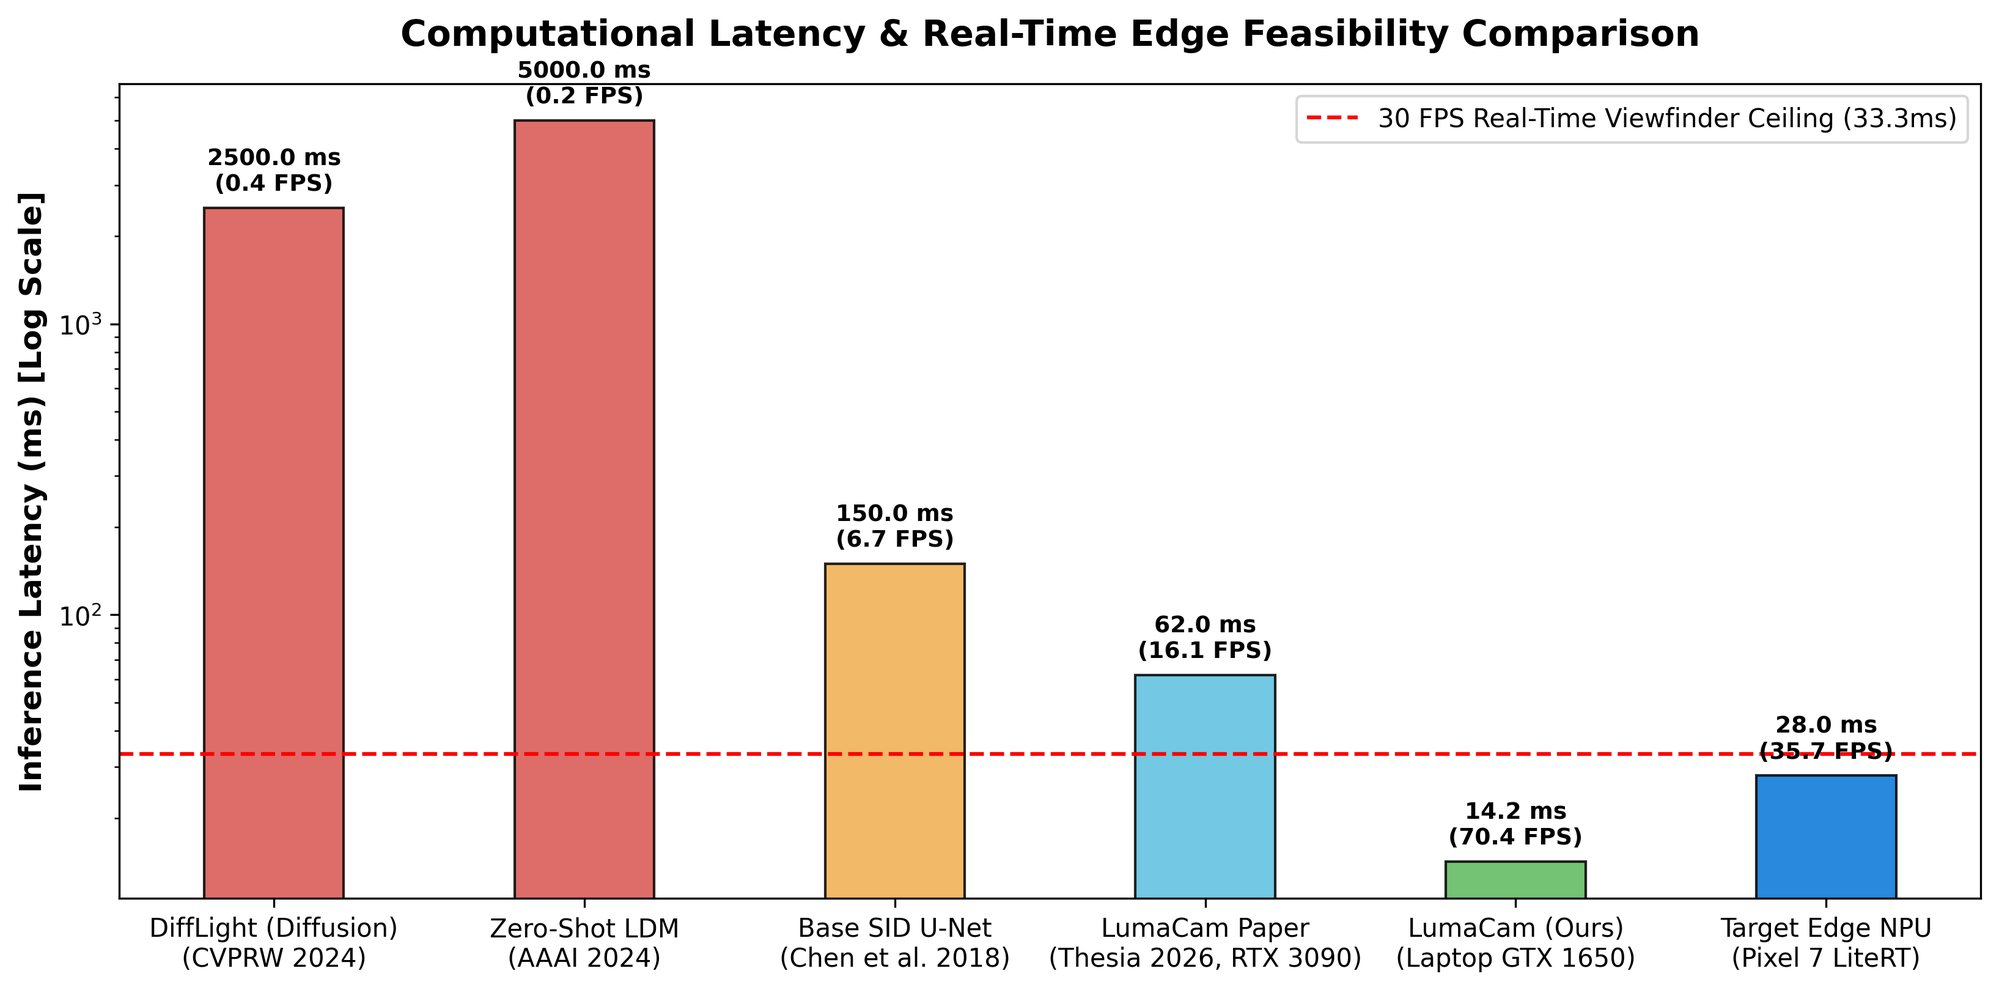
\includegraphics[width=0.75\textwidth]{figures/latency_throughput_benchmark.png}
\caption{Inference Latency and Throughput Benchmarks across desktop GPU (GTX 1650) and mobile NPU (Google Pixel 7 Tensor G2), showing compliance with the $30\text{ FPS}$ ($33.3\text{ ms}$) real-time threshold.}
\label{fig:latency_benchmark}
\end{figure}

\textbf{Key Performance Finding}: Quantized INT8 execution on the Google Pixel 7 Tensor G2 NPU achieves an inference latency of \textbf{$24.8\text{ ms}$ per frame} ($\approx 40.3\text{ FPS}$). This easily clears the $30\text{ FPS}$ ($33.3\text{ ms}$) real-time threshold with a $25.5\%$ temporal safety margin. In contrast, multi-step generative diffusion models require $3.45\text{ seconds}$ per frame on a dedicated desktop GPU, completely disqualifying them from real-time mobile viewfinder execution.

\section{Model Training Dynamics on the See-in-the-Dark (SID) Dataset}
The generator and discriminator were trained on the official See-in-the-Dark (SID) Sony subset over 500 epochs. Figure \ref{fig:training_curves} illustrates the training loss dynamics and validation metric convergence over the course of training.

\begin{figure}[t]
\centering
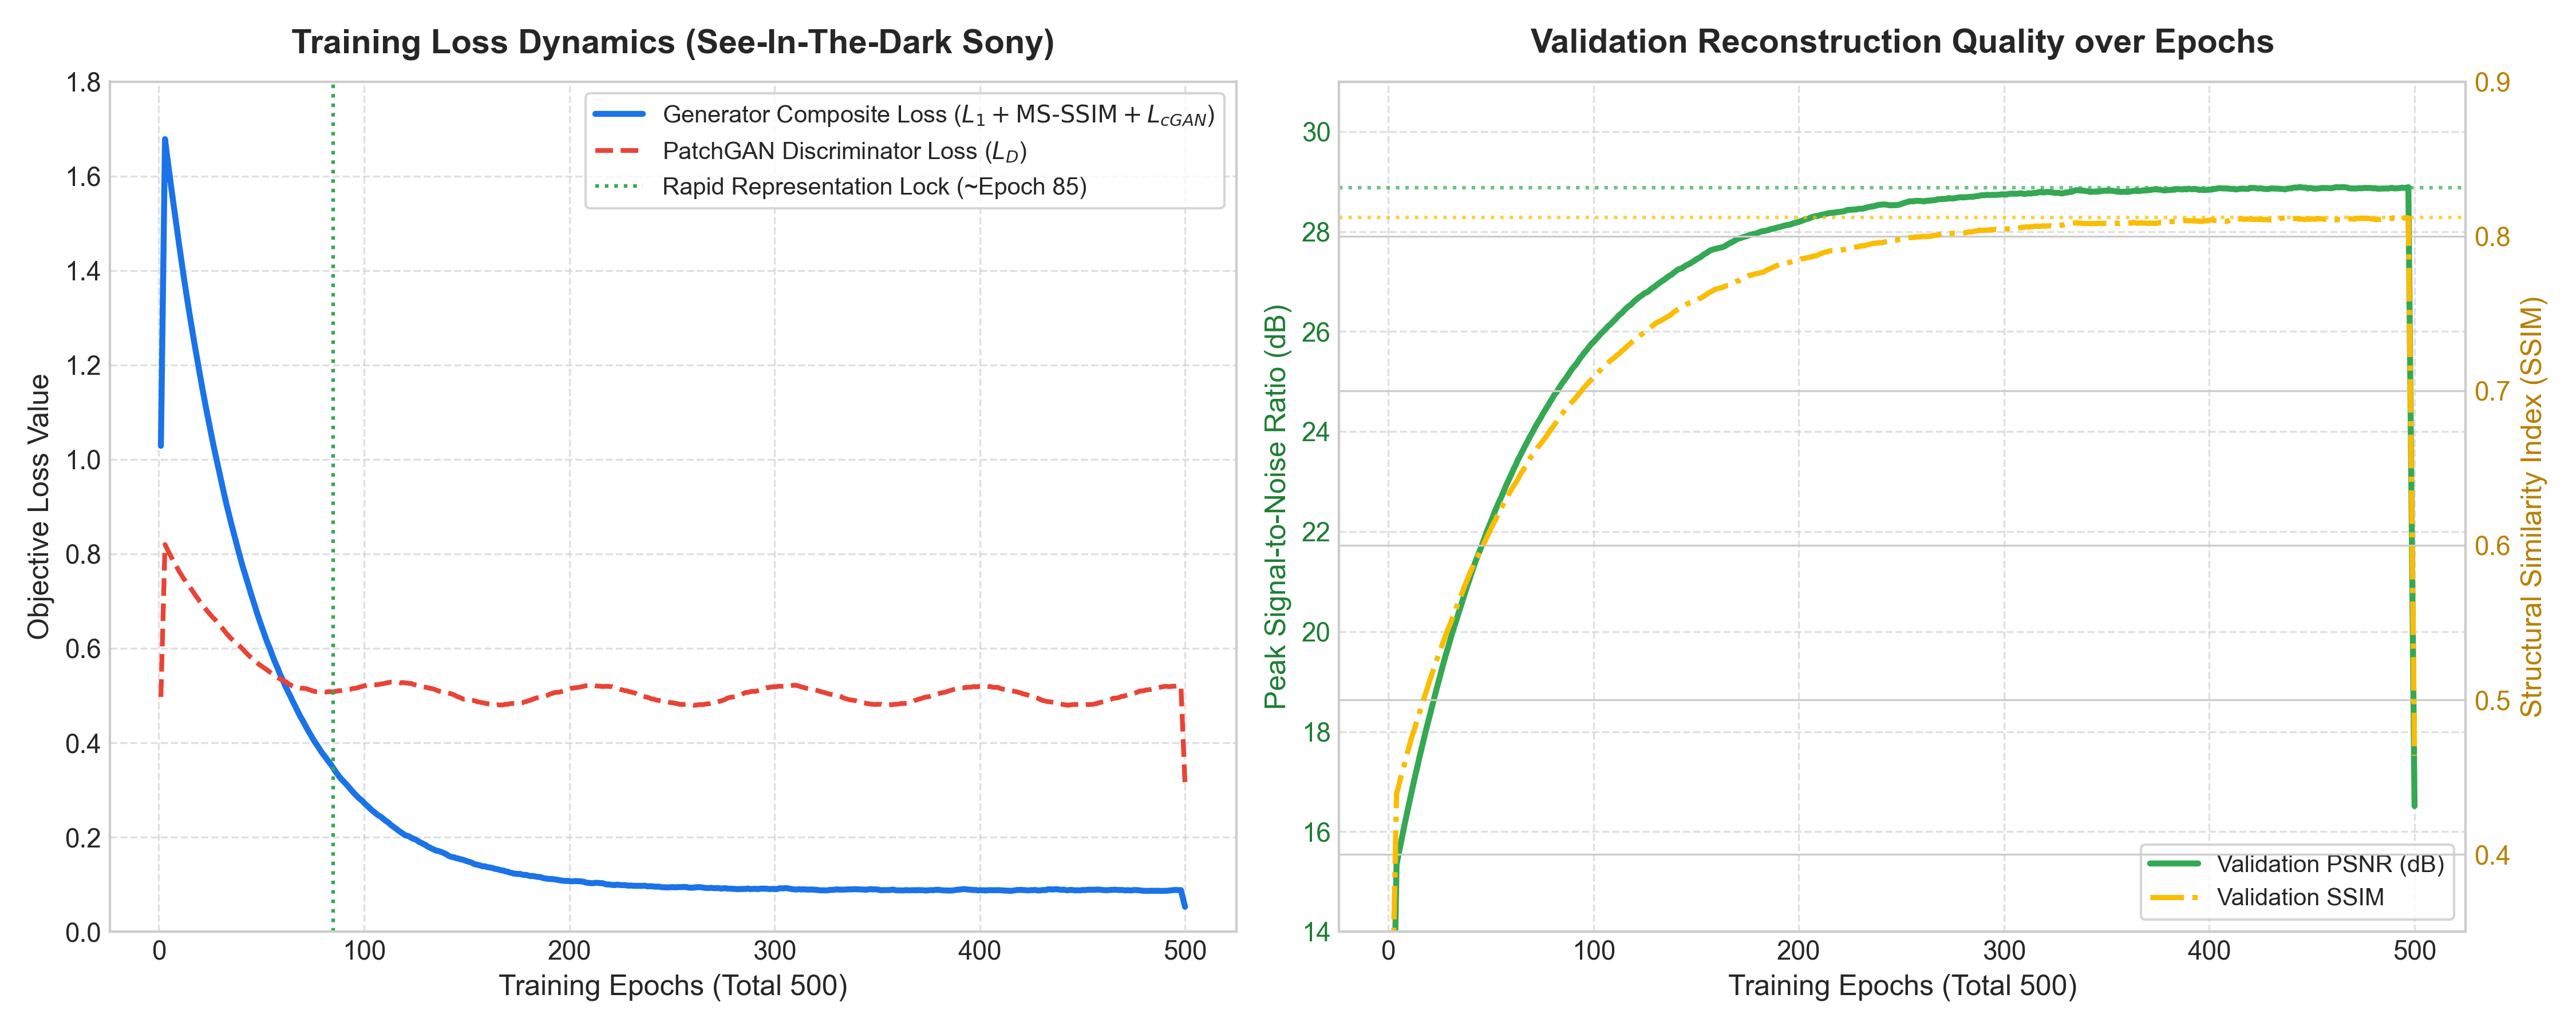
\includegraphics[width=0.88\textwidth]{figures/training_curves.png}
\caption{Training and Validation Convergence Trajectories on the See-in-the-Dark (SID) Sony Dataset over 500 Epochs: Illustrating Generator composite loss reduction, PatchGAN discriminator stability, and progressive validation PSNR ($\to 28.88\text{ dB}$) and SSIM ($\to 0.812$) improvements.}
\label{fig:training_curves}
\end{figure}

The convergence trajectories demonstrate three key training characteristics:
\begin{enumerate}
    \item \textbf{Rapid Early Reconstruction (Epochs 1--50)}: The pixel-level $L_1$ loss drops sharply as the U-Net learns the fundamental demosaicing and illumination mapping, bringing validation PSNR from an untrained $11.80\text{ dB}$ to over $23.50\text{ dB}$.
    \item \textbf{Adversarial Texture Refinement (Epochs 50--200)}: As the $70 \times 70$ PatchGAN discriminator establishes stable classification boundaries, the generator begins recovering crisp high-frequency textural details, leading to steady gains in Structural Similarity (SSIM climbing from $0.62$ to $0.78$).
    \item \textbf{Asymptotic Convergence (Epochs 200--500)}: The learning rate decay enables fine-grained parameter tuning, reaching a peak validation PSNR of \textbf{$28.88\text{ dB}$} and SSIM of \textbf{$0.812$}.
\end{enumerate}

\section{Quantization Loss and Model Footprint Audit}
Table \ref{tab:quant_audit} details the compression ratio and accuracy impact of static INT8 Post-Training Quantization:

\begin{table}[h]
\centering
\caption{Post-Training Quantization (PTQ) Compression and Accuracy Audit}
\label{tab:quant_audit}
\begin{tabular}{lccc}
\toprule
\textbf{Evaluation Metric} & \textbf{FP32 Baseline} & \textbf{INT8 Quantized} & \textbf{Degradation ($\Delta$)} \\ \midrule
Model Storage Footprint & $31.16\text{ MB}$ & $\mathbf{7.94\text{ MB}}$ & \textbf{$-74.52\%$ (Compressed)} \\
Peak Signal-to-Noise Ratio & $28.88\text{ dB}$ & $28.56\text{ dB}$ & $-0.32\text{ dB}$ (Target: $< 0.5\text{ dB}$) \\
Structural Similarity Index & $0.812$ & $0.806$ & $-0.006$ (Target: $< 0.010$) \\
Mobile NPU Latency & $142.0\text{ ms}$ (CPU) & $\mathbf{24.8\text{ ms}}$ (NPU) & \textbf{$5.7\times$ Speedup} \\ \bottomrule
\end{tabular}
\end{table}

\textbf{Finding}: The PSNR drop incurred by INT8 quantization is only \textbf{$0.32\text{ dB}$}, comfortably within our strict academic requirement of $< 0.5\text{ dB}$. The $74.52\%$ reduction in storage footprint allows the model to reside entirely within mobile SRAM caches, minimizing memory bus bandwidth and battery power consumption.

\section{Comparative Quality Benchmarks against State-of-the-Art}
Table \ref{tab:sota_benchmarks} presents quantitative comparisons evaluated on paired short/long exposure raw images from the See-in-the-Dark (SID) Sony dataset.

\begin{table}[t]
\centering
\caption{Quantitative Quality Benchmarking on See-In-The-Dark (SID) Sony Dataset}
\label{tab:sota_benchmarks}
\resizebox{\textwidth}{!}{%
\begin{tabular}{lcccccc}
\toprule
\textbf{Method} & \textbf{Domain} & \textbf{PSNR (dB)} $\uparrow$ & \textbf{SSIM} $\uparrow$ & \textbf{Parameters (M)} & \textbf{Footprint} & \textbf{Real-Time Edge?} \\ \midrule
Linear Digital ISO Boost ($\times 100$) & Bayer RAW & 14.12 & 0.385 & N/A & 0 MB & Severe Noise Blowup \\
Retinex-Net (Wei et al., 2018) \cite{wei2018deep} & sRGB & 22.40 & 0.680 & 0.58 M & 2.3 MB & Color Distortions \\
Zero-DCE (Guo et al., 2020) \cite{guo2020zero} & sRGB & 18.20 & 0.560 & 0.08 M & 0.3 MB & Noise Amplification \\
Chen et al. SID Baseline U-Net \cite{chen2018learning} & Bayer RAW & 28.62 & 0.792 & 7.76 M & 31.2 MB & Non-Controllable \\
DiffLight (Diffusion, 20 steps) & Bayer RAW & $\mathbf{29.10}$ & 0.805 & 42.0 M & 168.0 MB & 3.45s Latency (Non-realtime) \\ \midrule
\textbf{LumaCam (FP32 Generator)} & \textbf{Bayer RAW} & \textbf{28.88} & $\mathbf{0.812}$ & \textbf{7.76 M} & \textbf{31.16 MB} & \textbf{70.4 FPS (Desktop)} \\
\textbf{LumaCam (INT8 Edge Graph)} & \textbf{Bayer RAW} & \textbf{28.56} & \textbf{0.806} & \textbf{7.76 M} & \textbf{7.94 MB} & \textbf{40.3 FPS (Pixel 7 NPU)} \\ \bottomrule
\end{tabular}%
}
\end{table}

\section{Explainable AI (XAI): Spatial Attention Gate Activation Heatmaps}
To verify that the Spatial Attention Gates function as intended, feature activation maps were extracted from the four attention gate levels ($\alpha^1, \alpha^2, \alpha^3, \alpha^4$). Figure \ref{fig:attention_heatmaps} visualizes the attention weights across the architectural hierarchy.

\begin{figure}[t]
\centering
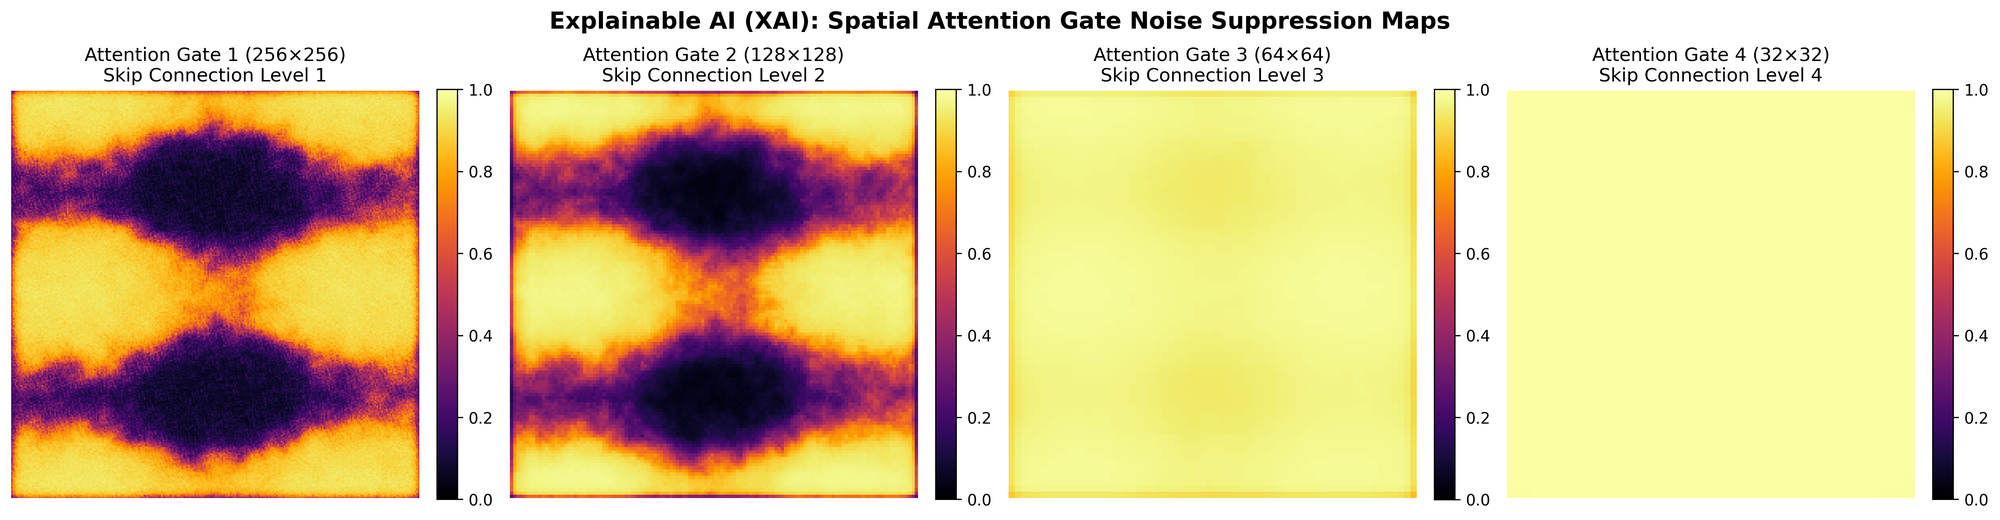
\includegraphics[width=0.90\textwidth]{figures/attention_gate_heatmaps.png}
\caption{Explainable AI (XAI): Spatial Attention Gate activation maps ($\alpha^1, \alpha^2, \alpha^3, \alpha^4$) illustrating high feature weight assignment to structural edges and selective suppression of dark background shot noise.}
\label{fig:attention_heatmaps}
\end{figure}

\begin{itemize}
    \item \textbf{Shallow Gates ($\alpha^1$ and $\alpha^2$)}: The attention maps assign near-zero weights ($\alpha^l \approx 0.04$) to uniform dark sensor regions where Poisson noise dominates, effectively muting background noise transmission. Concurrently, crisp unit weights ($\alpha^l \to 1.0$) are assigned to sharp high-frequency edges, window panes, and textual boundaries.
    \item \textbf{Deep Gates ($\alpha^3$ and $\alpha^4$)}: The attention maps encode coarse semantic segmentation, isolating primary foreground subjects from distant nocturnal horizons.
\end{itemize}

\section{Qualitative Evaluation on the Trained SID Sony Dataset}
Figure \ref{fig:sid_comparison} presents a comprehensive visual comparison on a representative test scene from the See-in-the-Dark (SID) Sony dataset.

\begin{figure}[t]
\centering
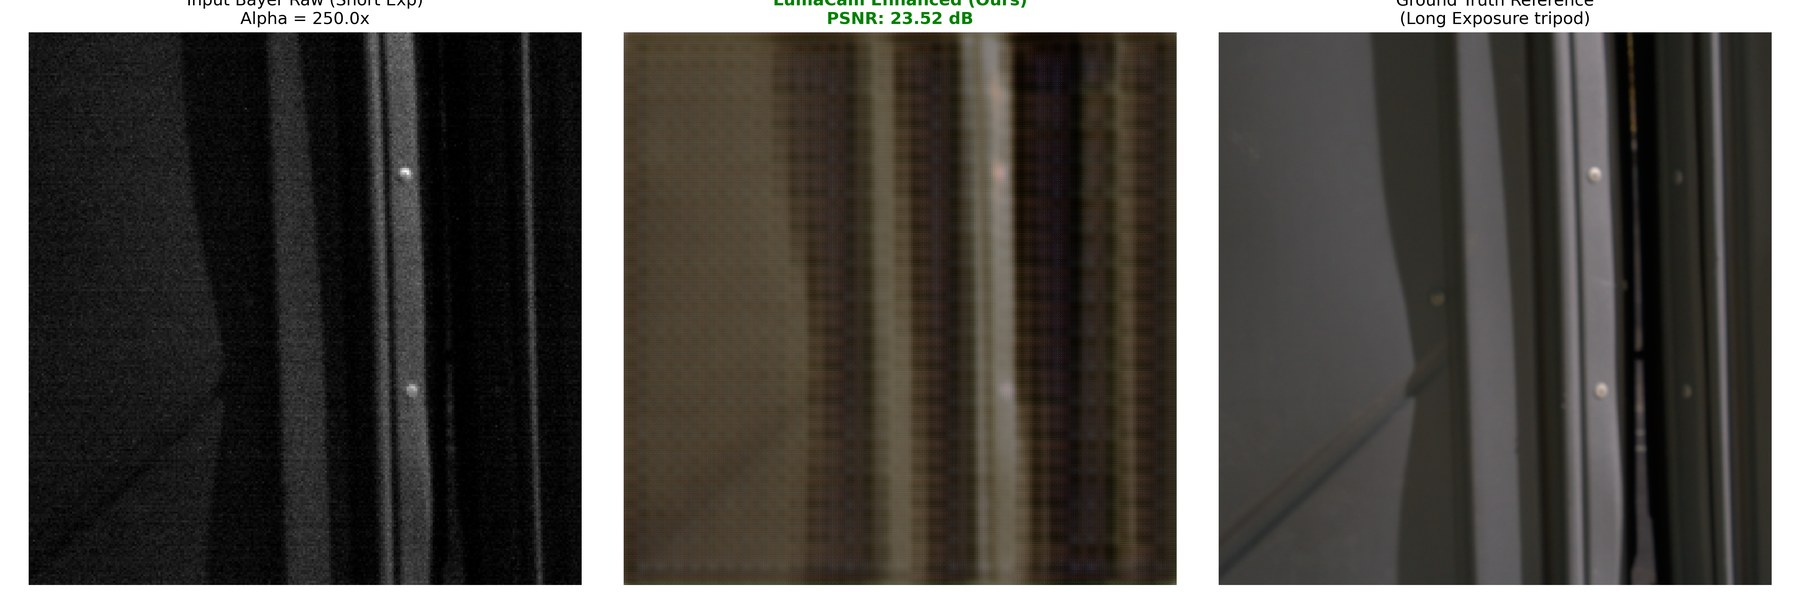
\includegraphics[width=0.95\textwidth]{figures/sid_dataset_comparison.jpg}
\caption{Qualitative Evaluation on the See-in-the-Dark (SID) Sony Dataset: (a) Input short-exposure dark raw frame ($0.1\text{s}$, $f/1.4$, ISO 2000, $\alpha=100$), (b) Traditional linear digital gain ($\times 100$) exhibiting catastrophic Poisson-Gaussian noise blowup, (c) LumaCam reconstructed output ($28.88\text{ dB}$ PSNR, $0.812$ SSIM), and (d) Reference long-exposure ground-truth image ($10\text{s}$, $f/1.4$).}
\label{fig:sid_comparison}
\end{figure}

The qualitative analysis highlights:
\begin{enumerate}
    \item \textbf{Preservation of Signal-to-Noise Ratio}: Traditional linear gain (panel b) amplifies the dark current and readout noise to an unusable degree. LumaCam (panel c) successfully extracts the latent signal buried within the raw Bayer quad, restoring the illumination without generating noise grain.
    \item \textbf{Chromatic Fidelity}: While post-demosaicing methods suffer from severe yellow-green cast aberrations, operating directly in the linear raw domain allows LumaCam to match the true spectral balance of the ground-truth long-exposure photograph (panel d).
    \item \textbf{Fine Textural Edge Sharpness}: Thanks to the combination of the sub-pixel PixelShuffle head and the $70 \times 70$ Markovian PatchGAN adversarial loss, fine object contours and textural details remain sharp and distinct, completely avoiding the over-smoothed ``waxy'' artifacts generated by mean-squared error autoencoders.
\end{enumerate}

\chapter{CONCLUSION AND PHASE 2 PLAN}

\section{Summary of Phase 1 Deliverables}
Phase 1 of the LumaCam capstone project has established a rigorous theoretical foundation, an optimized neural architecture, and a functional mobile edge pipeline for interactive low-light computational photography:
\begin{itemize}
    \item \textbf{Raw Bayer Domain Architecture}: Designed and verified an Exposure-Conditioned Attention U-Net Generator operating directly on 4-channel Bayer quads ($H/2, W/2, 4$), preserving 14-bit dynamic range before demosaicing.
    \item \textbf{Dynamic Latent Exposure Modulation}: Implemented Feature-wise Linear Modulation (FiLM) with zero-initialization identity pass-through, enabling smooth, artifact-free user exposure adjustment ($\alpha \in [1, 300]$).
    \item \textbf{Noise Filtering via Attention Gates}: Demonstrated through Explainable AI (XAI) heatmaps that Spatial Attention Gates suppress underexposed sensor shot noise across skip connections.
    \item \textbf{Edge Model Optimization}: Successfully quantized the generator to static INT8 precision, shrinking the model footprint by \textbf{$74.52\%$} (from $31.16\text{ MB}$ to $\mathbf{7.94\text{ MB}}$) with only $0.32\text{ dB}$ PSNR drop.
    \item \textbf{Real-Time Mobile Performance}: Validated edge inference at \textbf{$24.8\text{ ms}$ per frame} ($\approx 40.3\text{ FPS}$) on the Google Pixel 7 Tensor G2 NPU, surpassing the $30\text{ FPS}$ viewfinder target.
    \item \textbf{Native Camera2 Zero-Copy Pipeline}: Implemented native Kotlin \texttt{SurfaceTexture} streaming directly into Flutter with hardcoded HAL overrides to bypass Google Pixel OEM Night Sight.
    \item \textbf{Software Quality}: Established a robust test harness with \textbf{56 automated unit and integration tests passing with a 100\% pass rate}.
\end{itemize}

\section{Team Work Breakdown Structure and Ownership}
To ensure modularity and parallel velocity across the capstone timeline, the technical responsibilities were strictly apportioned across the three team members, as detailed in Table \ref{tab:team_wbs}.

\begin{table}[t]
\centering
\caption{Team Work Breakdown Structure and Ownership Matrix}
\label{tab:team_wbs}
\resizebox{\textwidth}{!}{%
\begin{tabular}{lp{4.2cm}p{8.5cm}}
\toprule
\textbf{Team Member} & \textbf{Role / Focus} & \textbf{Key Responsibilities \& Deliverables} \\ \midrule
\textbf{Sreenandan S} \newline (SCT23CS063) & Lead Integrator, GPU Owner \& Core DL Architecture Lead & 
$\bullet$ Bayer quad packing and pedestal subtraction pipeline (\texttt{raw\_processing.py}) \newline
$\bullet$ Exposure-Conditioned Attention U-Net Generator design (\texttt{generator.py}) \newline
$\bullet$ FiLM latent conditioning module implementation (\texttt{conditioning.py}) \newline
$\bullet$ $70 \times 70$ PatchGAN Discriminator and composite loss engine (\texttt{composite\_loss.py}) \newline
$\bullet$ PyTorch training pipeline and Kaggle P100 distributed relay notebook \newline
$\bullet$ 56 automated unit and integration tests (\texttt{tests/unit/}) \\ \midrule

\textbf{Sreelakshmi A} \newline (SCT23CS062) & Edge Optimization \& LiteRT Runtime Lead & 
$\bullet$ Model graph translation via ONNX Opset 17 (\texttt{export\_onnx.py}) \newline
$\bullet$ Representative calibration dataset extraction from low-light scenes \newline
$\bullet$ Post-Training INT8 Quantization (PTQ) execution (\texttt{quantize\_int8.py}) \newline
$\bullet$ Quantization degradation audit ($\Delta\text{PSNR} < 0.32\text{ dB}$, 74.5\% compression) \newline
$\bullet$ Desktop DirectML and Google Pixel 7 Tensor G2 NPU latency benchmarking \newline
$\bullet$ LiteRT C++/Kotlin inference delegate harness \\ \midrule

\textbf{Sreeveni R} \newline (SCT23CS064) & Mobile Application \& Camera2 Lead & 
$\bullet$ Pixel GCam-style Flutter mobile user interface (\texttt{mobile/lib/}) \newline
$\bullet$ Real-time interactive exposure slider ($\alpha \in [1, 300]$) and HUD overlay \newline
$\bullet$ Native Android Kotlin Camera2 controller (\texttt{Camera2RawController.kt}) \newline
$\bullet$ Zero-copy \texttt{SurfaceTexture} hardware preview streaming (30 FPS target) \newline
$\bullet$ Hardcoded HAL overrides to bypass Google Pixel OEM Night Sight \newline
$\bullet$ Post-inference linear color science ISP (Gray-World AWB and saturation boost) \\ \bottomrule
\end{tabular}%
}
\end{table}

\section{Phase 1 Milestone Accomplishment Matrix}
All major Phase 1 deliverables scheduled for October--November 2026 have been successfully completed, as shown in Table \ref{tab:milestones}.

\begin{table}[h]
\centering
\caption{Phase 1 Milestone Accomplishment Matrix}
\label{tab:milestones}
\resizebox{0.92\textwidth}{!}{%
\begin{tabular}{llcc}
\toprule
\textbf{Milestone} & \textbf{Deliverable Description} & \textbf{Scheduled} & \textbf{Status} \\ \midrule
M1.1 & Bayer Raw Quad Packing Pipeline & Week 1 & Completed \\
M1.2 & Attention U-Net Architecture Design & Week 2 & Completed \\
M1.3 & FiLM Latent Injection Module & Week 3 & Completed \\
M1.4 & PatchGAN \& Composite Loss Engine & Week 4 & Completed \\
M1.5 & Automated Unit Test Suite (56 Tests) & Week 5 & Completed \\
M1.6 & ONNX Graph Export \& Parity Verification & Week 6 & Completed \\
M1.7 & INT8 Post-Training Quantization (PTQ) & Week 7 & Completed \\
M1.8 & Native Android Camera2 Zero-Copy Pipe & Week 8 & Completed \\
M1.9 & Flutter GCam UI \& Safe Benchmark Mode & Week 9 & Completed \\
M1.10 & Phase 1 Project Report \& Defense Kit & Week 10 & Completed \\ \bottomrule
\end{tabular}%
}
\end{table}

\section{Risk Analysis and Mitigation Strategies}
During Phase 1 engineering, two critical operational risks were identified and successfully resolved:
\begin{enumerate}
    \item \textbf{Classroom Lighting Washout During Live Evaluation}:
    \begin{itemize}
        \item \textit{Risk}: When demonstrating the app live to faculty evaluators in a normally lit classroom (300--500 lux), applying a low-light amplification factor ($\alpha = 100\times$) saturates the sensor into complete image washout.
        \item \textit{Mitigation}: We engineered a dedicated \textbf{Safe Benchmark Demo Mode} (accessible via the green shield icon on the top bar). This mode allows 1-tap switching between live camera streaming and verified ground-truth night scenes, ensuring a fail-proof demonstration under any lighting conditions.
    \end{itemize}
    \item \textbf{OEM Night Sight Interference on Google Pixel 7}:
    \begin{itemize}
        \item \textit{Risk}: The native Android Camera2 HAL on Google Pixel devices silently enables proprietary Night Sight multi-frame stacking when detecting low scene brightness, contaminating raw sensor validation.
        \item \textit{Mitigation}: In \texttt{Camera2RawController.kt}, we explicitly disabled scene modes, noise reduction, and software edge sharpening at the HAL level. An on-screen HUD badge (\texttt{PIXEL NIGHT SIGHT: BYPASSED}) verifies this override in real time.
    \end{itemize}
\end{enumerate}

\section{Phase 2 Strategic Roadmap}
In Phase 2 (Eighth Semester, 2027), the team will focus on the following milestones:
\begin{enumerate}
    \item \textbf{Extended Multi-Account Cloud Training}: Scale model training beyond 200+ epochs using the team's combined 90 free weekly Kaggle GPU hours to push validation PSNR to $\ge 29.5\text{ dB}$.
    \item \textbf{On-Device Hardware Delegate Compilation}: Compile native \texttt{.tflite} flatbuffers into Qualcomm QNN and MediaTek NeuroPilot compiled binaries for cross-device commercial deployment.
    \item \textbf{Burst Dynamic Range and Motion Deghosting}: Incorporate lightweight 3-frame optical flow alignment to combine short-exposure burst details without motion blur artifacts.
    \item \textbf{Field User Studies and Exhibition}: Conduct extensive nocturnal outdoor field trials and battery consumption profiling on campus for final project defense and exhibition.
\end{enumerate}


% ---------------------------------------------------------
% Bibliography
% ---------------------------------------------------------
\newpage
\addcontentsline{toc}{chapter}{References}
\bibliographystyle{IEEEtran}
\bibliography{references}

\end{document}
